\section{Theoretical Foundation}
\label{sec:theoretical}

This section presents the fundamental concepts underpinning this research. It is organized
into four parts: general database concepts and the relational model; distributed database
systems; time series databases and their specific architectures; and benchmarking methodology.

\subsection{Databases}

According to~\cite{Ramakrishnan2003}, a database can be defined as a collection of data,
typically describing the activities of one or more related organizations. This encompasses
everything from information about entities (such as students and courses in a university)
to the relationships between those entities, such as student enrollments in specific courses.
\cite{Silberschatz2020} further argues that the primary goal of a database system must be to
provide a way of storing and retrieving information that is both convenient and efficient.

The management of this data is performed by a Database Management System (DBMS), which is
software designed to assist in the maintenance and use of large data collections~\citep{Ramakrishnan2003}.
The need for such systems has grown rapidly, as the alternative of storing data in flat files
and writing application-specific management code produces solutions that are not transferable
across applications and offer no guarantees of integrity or concurrent access safety.

As emphasized by~\cite{Ramakrishnan2003}, the success of an organization depends increasingly
on its ability to acquire accurate and timely data about its operations, manage that data
effectively, and use it to analyze and guide its activities. This positions the database as a
strategic organizational asset, not merely a technical component. \cite{Silberschatz2020} adds
that a database must provide users with an abstract view of the data, hiding the details of
storage and representation so it can serve as a practical problem-solving abstraction.

\cite{Ramakrishnan2003} enumerate several advantages of DBMSs over traditional file systems:
data independence (application programs are isolated from details of data representation and
storage); efficient data access (via sophisticated indexing and query optimization techniques);
data integrity and security (the DBMS enforces constraints and restricts unauthorized access);
and support for concurrent access and crash recovery.

The relational model, proposed by Codd in 1970, is simple and elegant: a database is viewed
as a collection of relations (tables with rows and columns), a representation so intuitive
that even non-specialist users can understand the stored content~\citep{Ramakrishnan2003}.
The structure of each relation consists of a schema (field names and their domains) and an
instance (the set of tuples, or records). A key property is that each relation is a set of
unique tuples, guaranteeing no duplicate records. Integrity constraints, defined as conditions specified
on the schema that restrict storable data, ensure that only valid database instances can
be persisted. Among these, primary key constraints uniquely identify tuples, while foreign key
constraints maintain consistency when information in one relation references another.

SQL became the commercial standard for interacting with relational databases.
As~\cite{Ramakrishnan2003} note, SQL is the most widely used commercial language for
relational DBMSs, supporting not only data definition and manipulation but also complex
querying. Database design typically begins with an Entity-Relationship (ER) diagram as a
high-level representation, which is then translated into a relational schema.

\subsection{Distributed Databases}

Distributed databases (DDBs) are the convergence of database systems technology and computer networks~\citep{Ozsu2011}. Database systems provide the mechanisms for data storage, querying, and integrity control,
while computer networks enable physical distribution across multiple nodes. DDB technology
combines these two fields, demonstrating that data integration does not necessarily imply
physical centralization.

For~\cite{Silberschatz2020}, a distributed database system is composed of multiple instances
with local databases, each capable of processing local transactions, while also executing
global transactions that access data across multiple sites, requiring inter-site communication.

A distributed database is defined as a collection of multiple logically inter-related databases
distributed over a computer network~\citep{Ozsu2011}. The distributed DBMS (DDBMS) is the
software that manages this distributed database, making the distribution transparent to users.
A DDB is not simply a collection of files stored on different network nodes; it is a structured
system with a defined schema accessible through a common interface.

The architecture of a DDBMS can take several forms, including client/server, peer-to-peer,
and multi-database systems~\citep{Ozsu2011}. In client/server systems, the functions are
divided between clients (managing the user interface) and servers (responsible for data
management). In peer-to-peer systems, all machines have full DBMS functionality and can
communicate directly. Multi-database systems deal with integrating heterogeneous and
autonomous databases.

A key benefit of DDBs is improved performance through data locality and parallelism. As~\cite{Ozsu2011}
note, storing data near its points of use reduces CPU and I/O contention, while parallelism
can be exploited both across queries (inter-query) and within a single query (intra-query).
However, this comes with challenges: replication consistency, distributed transaction
synchronization, and distributed deadlock detection, as highlighted by both~\cite{Ozsu2011}
and~\cite{Silberschatz2020}. The most important goal of database technology, as~\cite{Ozsu2011}
argue, is integration, not centralization.

\subsection{Time Series Databases}
\label{sec:tsdb-theory}

Time Series Databases (TSDBs) are a specialized category of storage systems designed to handle
data recorded as a sequence of values, each associated with a specific timestamp. According to
\cite{Ozsu2011}, a time series is a set of attribute values over a period of time. This
fundamental characteristic differentiates TSDBs from general-purpose databases: they are
optimized for time-interval-based queries, offering superior performance for that access pattern.

Weather records, economic indicators, and patient health metrics are all time series data.
Time series data also includes server metrics, application performance monitoring, network
data, sensor data, events, clicks, and many other types of analytical data~\citep{InfluxDataTimeSeries}.
Figure~\ref{fig:temporal_data} illustrates a time series of meteorological measurements.

\begin{figure}[ht]
  \centering
  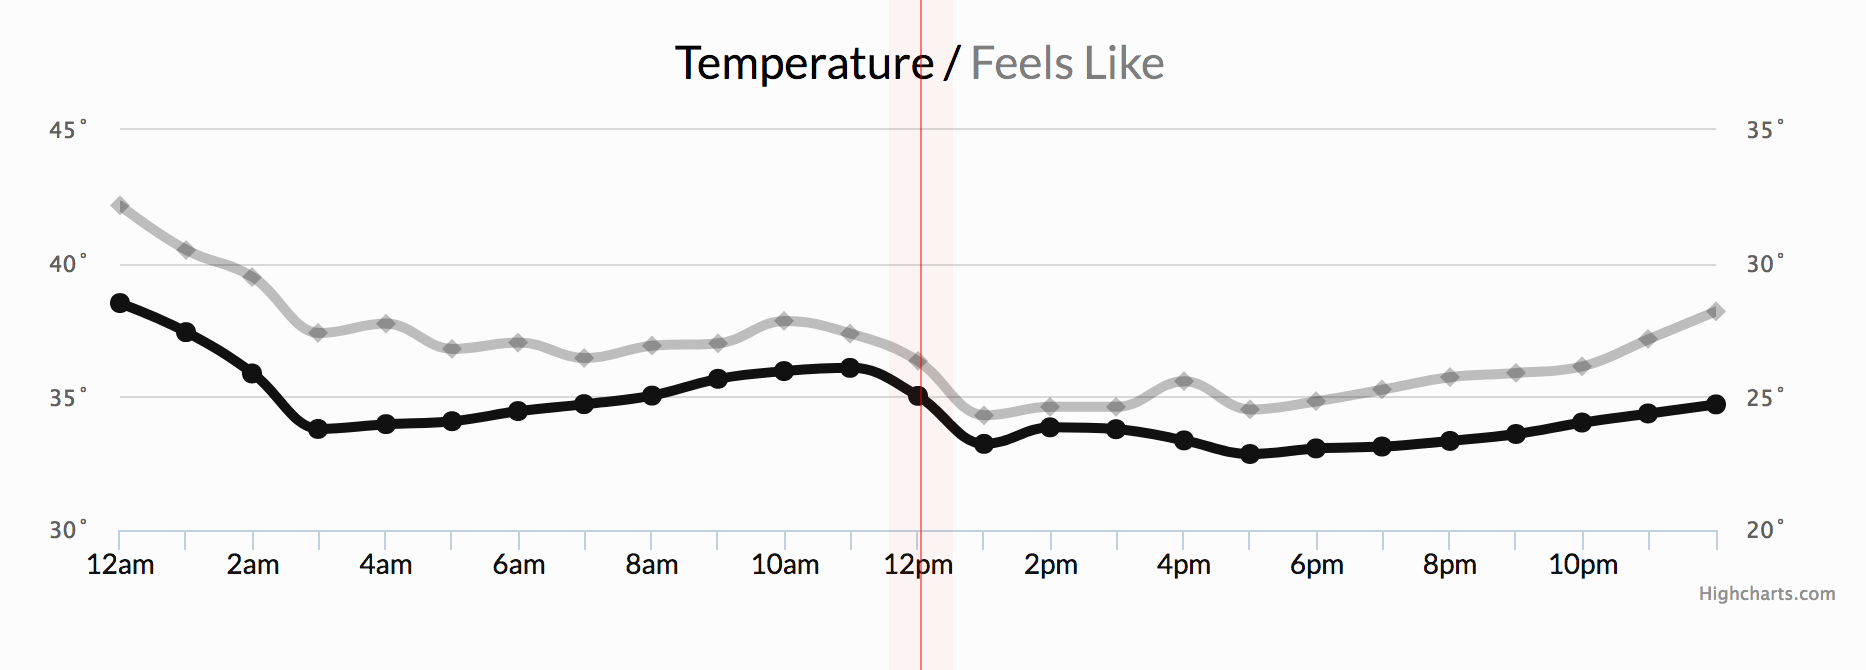
\includegraphics[width=\columnwidth]{figures/en_us/dado_temporal}
  \caption{Example of temporal data: weather conditions.
  The highlighted point represents a single data record captured at a specific instant.}
  \label{fig:temporal_data}
\end{figure}

\begin{figure}[ht]
  \centering
  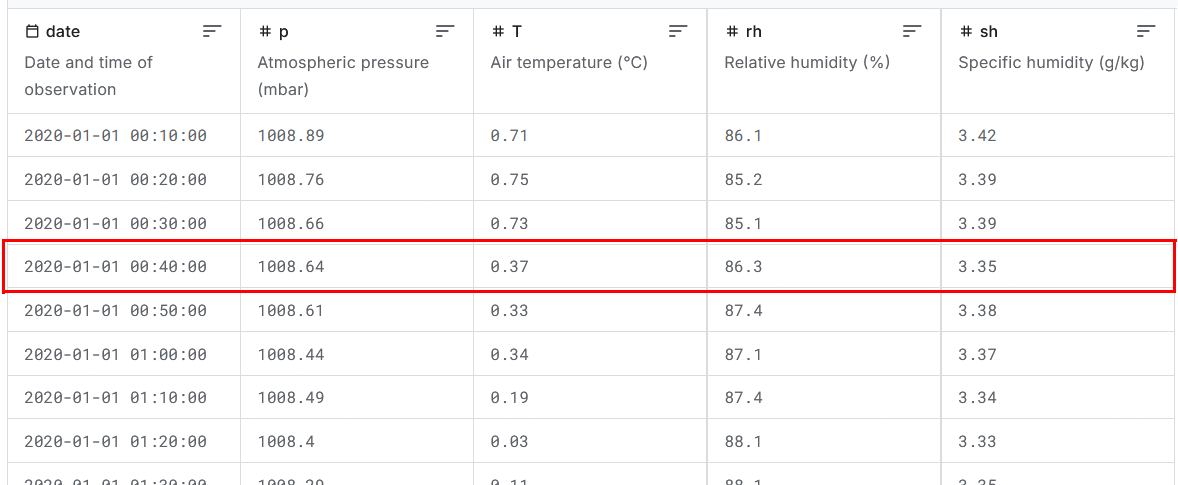
\includegraphics[width=\columnwidth]{figures/en_us/registro_temporal}
  \caption{Example of a TSDB table representing the weather time series.
  Each row corresponds to one time-indexed measurement.}
  \label{fig:tsdb_record}
\end{figure}

Figure~\ref{fig:tsdb_record} shows the corresponding TSDB table, where each row is a
time-indexed record capturing atmospheric pressure, temperature, humidity, and other readings
at a specific moment.

As explained by~\cite{Ozsu2011}, a time series normally consists only of numerical values,
either continuous or discrete. This makes it possible to model data streams that contain only
numerical values as time series, enabling time series analysis techniques to be applied to
certain types of data streams. A key characteristic is that time series datasets are typically
used in situations where measurements, once made, are not revised or updated but instead
accumulated; new data is added for each measured parameter at each new point in time,
as noted by~\cite{Dunning2014}.

The historical significance of time series analysis is remarkable, with examples dating back to
the 19th century. \cite{Dunning2014} cite the pioneering work of Matthew Fontaine Maury, who
analyzed ship logbooks to create wind and current charts, demonstrating how the collective
analysis of time series data accumulated over many years across many ships can reveal patterns
valuable for maritime navigation. This historical example illustrates how time series datasets
can reveal trends and patterns not apparent in point-in-time measurements.

In the modern context, TSDBs face new challenges due to the volume, velocity, and variety of
generated data. What used to be collected in 10 minutes for some very active systems is now
generated every second~\citep{Dunning2014}. This explosion in data volume demands new approaches
to storage and access, making NoSQL databases particularly suitable for this scale. For
time-based queries at very large scales, these accesses can be implemented as large, contiguous
scans that are highly efficient if data is stored appropriately in a time series database.

The architecture of modern TSDBs has evolved considerably. \cite{Dunning2014} describe three
main approaches to time series storage: (1) wide tables that store data point-by-point;
(2) a hybrid design mixing wide tables with blob storage; and (3) direct blob insertion from
a memory cache, which can achieve ingestion rates up to 1{,}000$\times$ faster than
point-by-point approaches. TSDBs store multiple time series in such a way that queries
retrieving data from one or a few series for a specific time interval are particularly
efficient~\citep{Dunning2014}. This efficiency is achieved through storage strategies that group
temporally proximate data physically, enabling efficient sequential scan operations.

Applications of TSDBs are diverse and expanding. In the financial sector, the speed of trading
and the need for extremely low latency make high-performance TSDBs essential~\citep{Dunning2014}.
In the IoT context, TSDBs occupy a central position in the sensor-to-insight data flow that is
rapidly changing how we perceive and understand the world~\citep{Dunning2014}.

\subsubsection{Database Architectures for Time Series}

The three databases compared in this work represent three distinct storage architectures for
time series data, each with different trade-offs between write throughput, read latency, and
resource consumption.

\textbf{Apache IoTDB}~\cite{wang2023iotdb} is purpose-built for the IoT domain. It uses TsFile~\citep{zhao2024tsfile},
a custom columnar file format that stores data in sorted chunks with per-chunk min/max statistics.
Writes are first absorbed into an in-memory buffer (memtable) managed by the JVM, and are
flushed to TsFile segments asynchronously. This deferred write strategy is similar to a
Log-Structured Merge Tree (LSM) approach~\citep{oneil1996lsm}, trading strict durability guarantees for high
write throughput. The native ingestion interface is a binary Thrift RPC protocol
(SESSION\_BY\_TABLET), which submits typed columnar tablets directly into the write buffer
with minimal overhead. The min/max statistics stored per chunk enable early pruning of
non-matching blocks during value-predicate queries, a property that becomes increasingly
advantageous as the dataset grows~\citep{wang2023iotdb}.

\textbf{InfluxDB}~\cite{naqvi2017influxdb} uses a Time-Structured Merge Tree (TSM) storage
engine, which organizes data into compressed time-ordered blocks. Like the LSM tree, TSM
buffers incoming writes in memory (the TSM cache) and periodically compacts them into
immutable on-disk files. Data ingestion is performed via an HTTP line-protocol API, where
clients POST line-protocol text representing measurements. Queries use the Flux language.
The TSM engine maintains a Time Series Index (TSI) for series lookup. InfluxDB's in-process
memory is dominated by the TSM cache, the series index, and Go runtime overhead~\citep{naqvi2017influxdb}.

\textbf{TimescaleDB} extends PostgreSQL with time-series optimizations~\citep{timescaledb}.
Its primary data structure is the \textit{hypertable}: a logical table that is automatically
partitioned into physical \textit{chunks} by time interval. Queries that specify a time range
can prune chunks automatically, touching only the relevant partitions. The \texttt{time\_bucket()}
function provides native downsampling with push-down aggregation. As a PostgreSQL extension,
TimescaleDB inherits its full storage stack: all writes go through the Write-Ahead Log (WAL)
before acknowledgement, MVCC provides snapshot isolation, and B-tree indexes are maintained
on primary and secondary columns. BRIN (Block Range INdex) indexes provide lightweight
range-based pruning for value predicates. The WAL-based durability model provides strong
data safety guarantees but introduces higher per-write latency compared to the asynchronous
buffering of IoTDB and InfluxDB.

\subsection{Benchmarks}

Performance evaluation is a critical component of the database selection process.
As highlighted by~\cite{Ramakrishnan2003}, when a database grows beyond the capacity of its
current DBMS to provide satisfactory performance, migration to a new system must be considered.
Benchmarks are the primary tools that enable objective comparison between the different products
available. A single test is insufficient; as~\cite{Silberschatz2020} argues, a benchmark must
simulate real workloads because each product may perform differently depending on the task.

The complexity of DBMSs and the different approaches adopted by vendors make benchmarks
particularly valuable. As~\cite{Ramakrishnan2003} observe, a DBMS is complex software, and
different vendors may target different market segments, optimizing certain parts of their
systems or choosing different architectural designs. This diversity of approaches and
specific optimizations makes direct comparison difficult without standardized instruments.

Regarding the fundamental characteristics of a good benchmark,~\cite{Ramakrishnan2003} enumerate
three essential qualities. First, \textit{portability}: the ability to run the benchmark on
different platforms and systems. Second, \textit{clarity}: ensuring easy understanding of what
is actually being measured. Third, \textit{scalability}: the natural adaptation to larger
problem instances. Beyond these basic attributes, good benchmarks should measure both maximum
performance (expressed in metrics such as transactions per second) and cost-effectiveness
(dollars per transaction per second) for workloads typical of a specific application domain.
It was precisely to meet these needs that the Transaction Processing Council (TPC) was created,
with the mission of developing standardized benchmarks for transaction processing and database systems.

\cite{Silberschatz2020} adds an important note on correct performance calculation: using
the simple average of throughputs can be misleading. The proper method is to calculate the
total time for a mixed workload and derive the average throughput from that, or to use the
harmonic mean, which better reflects the reality when there are different types of operations.

The benchmark literature categorizes its instruments in several groups~\citep{Ramakrishnan2003}.
\textit{Online Transaction Processing} benchmarks (TPC-A, TPC-B, TPC-C) define standard
measures for transactions per second and cost per transaction. TPC-C, the most widely used,
models a complex warehouse environment with five transaction types, exercising a much broader
range of system capabilities than its predecessors. \textit{Query performance} benchmarks
(Wisconsin, AS3AP, TPC-D) evaluate relational query performance from simple to complex
decision-support workloads. \textit{Object database} benchmarks (001, 007, Bucky) measure
object-oriented and object-relational systems.

For practical application, benchmarks must be interpreted carefully.
\cite{Ramakrishnan2003} caution that single-number performance metrics can be oversimplistic
for complex software like a DBMS. A good benchmark should include a comprehensive suite of
tasks carefully selected to cover a specific application domain and to test the DBMS capabilities
critical for that domain. Analysts should weight benchmark tasks according to how closely they
resemble the critical operations of the intended application; and when standard benchmarks
do not match the actual workload closely enough, custom benchmarks that adapt or replace
standard tasks with more representative operations should be considered.

Reproducibility is an essential but often neglected property of database benchmarks.
Among the six performance studies reviewed in this work, only one provides the scripts
and exact configurations needed for independent
replication~\citep{pereira2023mulletbench}. This limits the ability to validate results,
compare findings across studies, and build on prior work, a gap this study directly
addresses through its fully scripted and publicly available benchmark infrastructure.
Beyond code sharing, resource isolation between benchmark systems is equally critical:
running multiple database engines on shared hardware introduces page-cache and I/O
contention artefacts that can reverse reported conclusions~\citep{shapira2016pitfalls}.
